\section{Standard Persistent Homology}
\label{section-standard}

We begin by describing persistent homology over a field for finite simplicial complexes. These conditions allow a complete characterisation of the persistent homology of a filtration via simple combinatorial objects called barcodes. In practice, because our data is finite, we always deal with finite simplicial complexes. Algorithms exist to compute the barcode of a filtration of a simplicial complex.

\subsection{Persistent homology groups}

A filtration is a way of gradually building up a topological space. We can extend our definition of homology to apply to each intermediate space in a filtration. Because our filtration is finite, without loss of generality we consider filtrations indexed by the natural numbers.

First, fix a dimension $n$ and consider all homology to be done at this dimension. Let $K$ be a filtration and let $H_i$ denote the homology of the space $K_i$.

If we wish to use a filtration to find topological features of a space, we might consider, for example, the sequence of Betti numbers produced by moving up the filtration. Unfortunately, from these alone there is no way to distinguish true features of the space from the noise caused by our construction of the filtration.

In any filtration there are inclusion maps $\iota_i^j : K_i \to K_j$ for any $i \leq j$. By Theorem~\ref{homology-functor}, each induces a homomorphism $\eta_i^j : H_i \to H_j$. When we move to the right in this sequence, we could gain homology classes or lose some as they become trivial or merge together.

The idea behind persistence is that any significant topological feature of the data should exist along a large interval of the filtration. This leads us to define the persistent homology groups of our filtration, which will represent homology classes in each space that still exist some number of spaces later in the filtration.

\begin{definition}[Persistent homology]
Let $K_i$ be a filtration. The \emph{persistent homology groups of $K$}, denoted $H_i^j$, are the images of the induced homomorphisms $\eta_i^j$.
\end{definition}

These groups consist of the homology classes of $K_i$ that are still ``alive'' in $K_j$. An alternative definition is to factor out the cycle group of $K_i$ by the boundary group of $K_j$:
\begin{align*}
H_i^j = Z_i / (B_j \cap Z_i).
\end{align*}
Both $B_j$ and $Z_i$ are subgroups of $C_j$, so the intersection $B_j \cap Z_i$ is well-defined.

We can also track the lifetime of an individual homology class. Let $\gamma \in H_i$. We say $\gamma$ is \emph{born at $K_i$} if it first appears in $K_i$, i.e., $\gamma \notin H_{i-1}^i$. The class \emph{dies entering $K_j$} if it merges with an older class when we move from $K_{j-1}$ to $K_j$. That is,
\begin{enumerate}
\item $\eta_i^{j-1}(\gamma) \notin H_{i-1}^{j-1}$ ($\gamma$ in $K_{j-1}$ is not the image of a class in $K_{i-1}$); but,
\item $\eta_i^j(\gamma) \in H_{i-1}^j$ ($\gamma$ in $K_{j}$ is the image of a class in $K_{i-1}$).
\end{enumerate}

The \emph{lifetime} of a homology class $\gamma$ is the half-open interval $[i, j)$, where $\gamma$ is born at $K_i$ and dies entering $K_j$. If $\gamma$ is born at $K_i$ but then never dies, its lifetime is $[i, \infty)$.

\begin{example}
Consider the filtration given earlier as Figure~\ref{fig:filtration}. The homology class $\sigma = [a, b] + [b, d] - [a, d]$ is born at stage $K_3$, as it is not the image of a homology class in any earlier $K_i$. It dies one step later in $K_4$, as the class becomes trivial. The lifetime of $\sigma$ is therefore $[3, 4)$.
\end{example}

\subsection{Persistence modules}

At this point it is not clear whether we can get a succinct description of the persistent homology of a filtration. In their foundational paper, Zomorodian and Carlsson \cite{zomorodian2005computing} showed that a description exists for finite simplicial complexes when the homology coefficient ring is a field.

Intuitively, computing persistent homology requires us to find compatible bases for $H_i$ and $H_j$. We begin by constructing one large structure that contains the homology groups for all steps in the filtration.

\begin{definition}
A \emph{persistence module} $\mathcal{M}$ is a family of $R$-modules $\{ M_i \}_{i \geq 0}$ together with module maps $\varphi_i : M_i \to M_{i+1}$.
\end{definition}

The set of homology groups $H_i$ form a persistence module, with the maps $\varphi_i$ induced by the inclusion maps $K_i \to K_{i+1}$.

Given a persistence module, we can construct a single graded module that contains the same data. Let $\mathcal{M} = \{M_i, \varphi_i\}$ be a persistence module over the ring $R$. Now define the graded module over $R[t]$:
\begin{align*}
  \alpha(\mathcal{M}) = \bigoplus_{i=0}^\infty M_i,
\end{align*}
where the action of $R$ is just the action on each component, and the action of $t$ is
\begin{align*}
t \cdot (m_0, m_1, m_2, \dots) = (0, \varphi_0(m_0), \varphi_1(m_1), \varphi_2(m_2), \dots).
\end{align*}

In homology terms, multiplication by $t$ moves a homology class up the filtration by one. If some homology class $\gamma$ exists in $K_i$, then $t \cdot \gamma$ is an element of $K_{i+1}$.

\begin{definition}
A graded module $R[t]$ is of \emph{finite type} if each $M_n$ is finite dimensional over $R$.
\end{definition}

Because our filtration is finite, its homology is also finite and therefore the graded $R[t]$ module will be of finite type.

\begin{theorem}[Correspondence]
The map $\alpha$ is a one-to-one correspondence between the set of persistence modules over $R$ and the set of graded modules of finite type over $R[t]$.
\end{theorem}
\begin{proof}
We construct an inverse to $\alpha$ in the obvious way. If $G$ is a graded module of finite type over $R[t]$, let $M_i$ be the submodule of $G$ with grading $i$ considered as a $R$-module and set $\varphi_i(a) = t \cdot a \in M_{i+1}$.
\end{proof}

From this we learn there is little hope for a simple classification of persistence modules when the ground ring is not a field. Even in the simple case of $R=\mathbf{Z}$, $\mathbf{Z}[t]$-modules are known to be extremely difficult to classify.

When $R$ is a field $\mathbf{k}$, the graded ring $\mathbf{k}[t]$ is a PID, so we can classify the persistence modules using Theorem~\ref{thm:graded-pid-structure}, the structure theorem for graded modules over PIDs. The only graded ideals of $\mathbf{k}[t]$ are homogeneous of the form $\langle t^n \rangle$, so
\begin{align*}
\alpha(\mathcal{M}) \cong \left( \bigoplus_{i=1}^n \Sigma^{\alpha_i} \mathbf{k}[t] \right) \oplus \left( \bigoplus_{i=1}^m \Sigma^{\beta_i} \mathbf{k}[t] / \langle t^{n_i} \rangle \right).
\end{align*}

Remember that $\Sigma^k$ represents an upward shift of $k$ steps in the grading.

This decomposition holds the description for persistence that we seek. In the first sum, the free part, each summand gives a class $\gamma$ that first appears at time $\alpha_i$, and $t \cdot \gamma, t^2 \cdot \gamma, \dots$ remain nonzero for all steps in the filtration after that. This corresponds to a persistence interval of $[\alpha_i, \infty)$.

In the second sum, the torsion part, a class $\tau$ first appears at time $\beta_i$, and exists as $t \cdot \tau, t^2 \cdot \tau, ..., t^{n_i-1} \cdot \tau$. After this, $t^{n_i}$ becomes zero, so our homology class is mapped to zero at time $\beta_i + n_i$. This gives us an interval $[\beta_i, \beta_i + n_i)$.

These sets of intervals are known as \emph{barcodes}. More precisely:

\begin{definition}
A \emph{barcode} is a finite multiset of ordered pairs $(i, j)$, with $0 \leq i < j$, and $i, j \in \mathbb{Z} \cup \{\infty\}$.
\end{definition}

The barcode exactly determines the structure of a $\mathbf{k}[t]$-module, so we can restate the correspondence as follows:

\begin{corollary}
There is a bijective correspondence between barcodes and persistence modules of finite type over a field.
\end{corollary}

\begin{example}
Let us return to the filtration shown in Figure~\ref{fig:filtration} and compute the barcode for the 0-dimensional homology. The space $K_1$ introduces two new components, so two new homology classes. Both classes are mapped into the same component in $K_2$, so one of the classes dies entering $K_2$. An additional class is born in $K_2$, which then joins the rest of the  space in $K_3$. The barcode is therefore $\{[1,2), [1, \infty), [2, 3)\}$.

Similarly, two 1-dimensional homology classes are created in $K_3$. In $K_4$, one of these becomes trivial. The barcode is then $\{[3, 4), [3, \infty) \}$.
\end{example}

Barcodes can be represented pictorially by simply plotting each interval $[p, q)$ as a point $(p, q)$ in the plane. This set of points must lie above the line $x = y$. Features with short lifetimes will correspond to points that lie close to the diagonal.

\begin{figure}
\centering
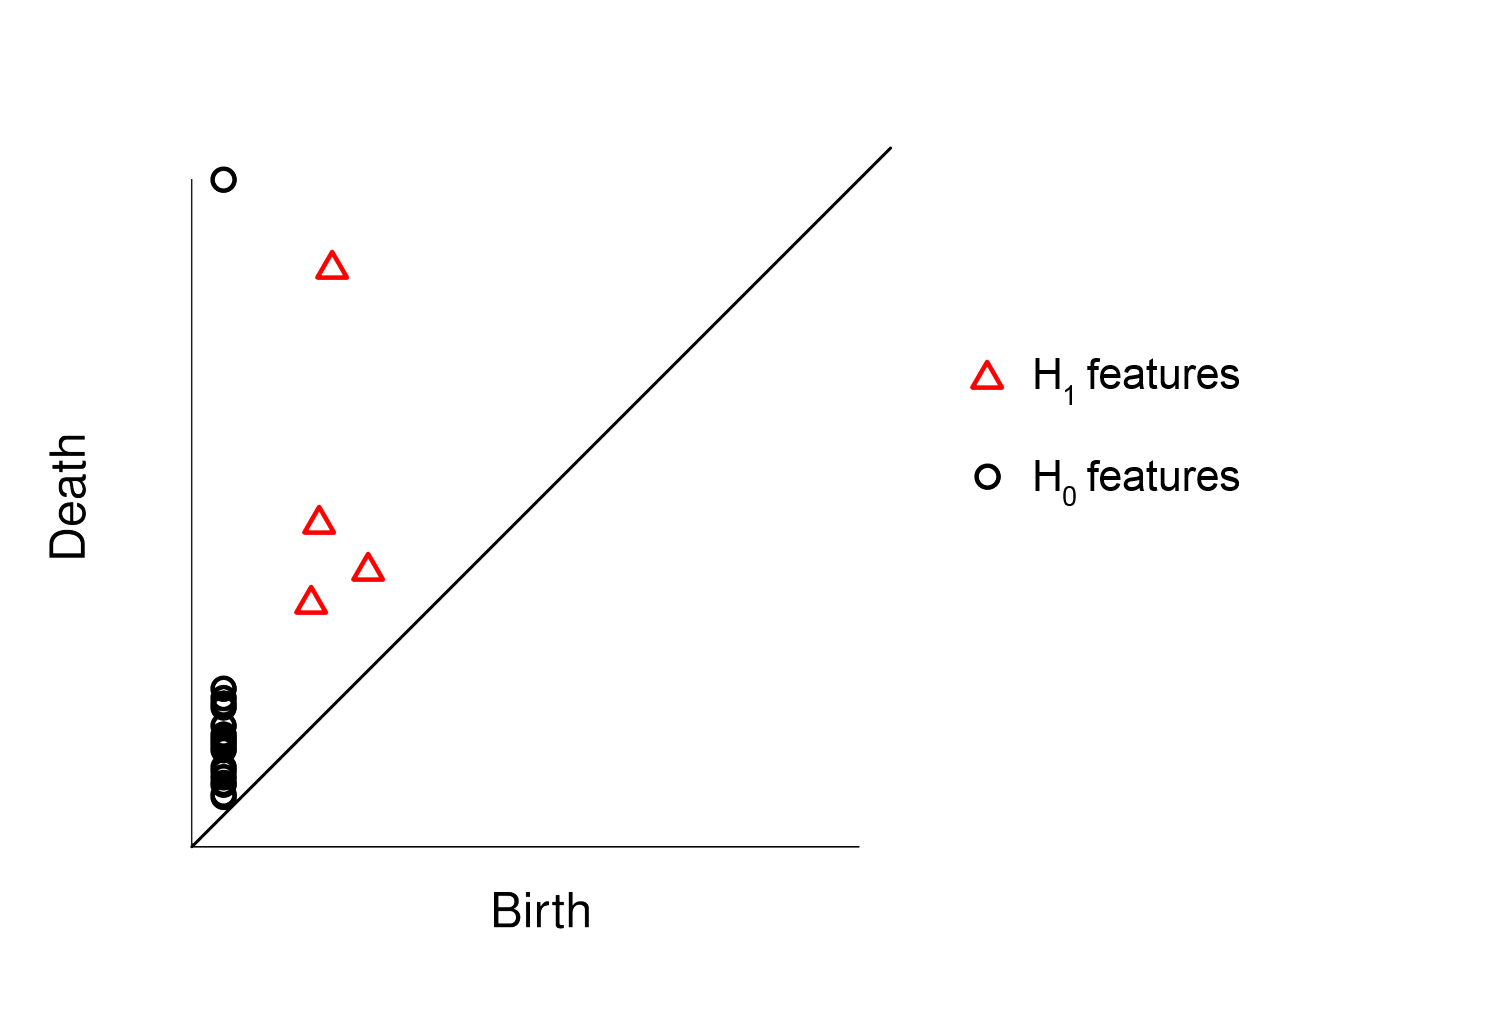
\includegraphics[scale=0.3]{diagram.png}

\caption{A sample persistence diagram}
\label{fig:examplediagram}
\end{figure}

\subsection{Algorithms}

Zomorodian and Carlsson also provide an algorithm to systematically calculate the barcode of an input filtration. Appendix~\ref{code-appendix} contains a Haskell implementation of the algorithm, completed as part of this project. Haskell was chosen as it is well suited for defining mathematical objects such as simplices, groups, vector spaces, and so on.

The algorithm has since been improved in a number of ways. Most notably, calculating persistent cohomology \cite{de2011dualities} has been shown to have much better performance in practice. Poincar\'e duality implies that over $\mathbb{Z}/2\mathbb{Z}$, the barcodes produced this way are the same as would be produced by persistent homology.